\chapter{Introdução}
\label{chp:introduction}

O curso de Tecnologia em Sistemas para Internet (TSI) do \ac{ifb} tem as etapas de qualificação e defesa do \ac{tcc} bem como suas respectivas disciplinas do 4º e 5º semestre, tidas como requisitos obrigatórios previstos no \ac{ppc} para obtenção de obtenção da diplomação como tecnólogo.

O documento apresentado a seguir visa descrever os principais elementos que compõem a qualificação e defesa do projeto auxiliando os alunos das disciplinas de trabalho conclusão de curso em Sistemas de Informação do IFB campus Brasília na compreensão lógica e construção dos documentos que fazem parte destas etapas.

Ele foi elaborado em LaTex, que segundo \textit{\ac{ctan}} é um "sistema de composição tipográfica"  \citep{ctan} que incorpora um processador de macro onde objetos e textos são compilados gerando como saída um arquivo no formato .pdf. Caso você identifique algum então fora da norma, registre para contribuir e traga para a disciplina pois este documento está sendo revisado em conjunto com a biblioteca e outros professores para que o formato siga todos os padrões da ABNT quanto a sua formatação. 

Para elaboração do trabalho, caso o estudante prefira, também pode se utilizar o modelo de trabalho acadêmico em MS-Word.
\url{https://drive.google.com/file/d/1KBzPjuZpI-B8hSV0xOWzNf-L8C7ZkfSL/view} disponibilizado pelo IFB no site normaliza. 


\section{Mas o que é um TCC?}

O trabalho de conclusão de curso é um relato, uma história que conta o que você aprendeu durante o curso e como isso demonstra as competências da sua formação profissional e acadêmica. Esse relato tem algumas características específicas no método e forma de construção e avaliação sendo importante destacar alguns pontos sobre a sua condução e lógica de escrita.

Fato do seu relato contar uma história não quer dizer, por exemplo, que você vai criar um suspense ou fazer uma propaganda exagerada do tema do trabalho. Na estrutura do texto e encadeamento de ideias você deve ser o mais direto e objetivo possível trazendo para o texto explicações, ou pelo menos um resumo sobre os assuntos e os termos que você deseja trabalhar no projeto assim que eles são tratados.

O objetivo geral de um trabalho de conclusão de curso é servir como um registro técnico de onde (contexto), porque  justificativa e objetivos), como (método) e oque (resultados e conclusões) você fez para resolver ou melhorar uma determinada situação.O trabalho é dividido em duas etapas (qualificação e defesa) que acontecem nos dois semestre do curso. 

A etapa de qualificação busca apresentar para banca um projeto onde é possível, para os membros da banca, perceber principalmente: a escolha do tema e uma justificativa plausível para desenvolvimento de trabalho; o conhecimento sobre as tecnologias e suas relações com a solução do problema proposto ou objetivos a serem alcançados; e um cronograma exequível de implementação da solução. 

O trabalho da banca é avaliar a qualidade do texto produzido e o conhecimento dos alunos sobre o contexto e tecnologias envolvidas no projeto ou que serão aprendidas e a viabilidade de desenvolvimento do projeto na fase de qualificação.

A etapa de defesa do trabalho os alunos buscam apresentar para banca as melhorias vindas da etapa de qualificação e o desenvolvimento do projeto que foi aprovado na etapa anterior. Este desenvolvimento abrange a descrição das diversas atividades executadas, a produção de artefatos, sejam estes documentos, linhas de código e implementações e testes destas. 

A partir dos resultados é possível identificar como e quais objetivos específicos foram alcançados e os seus impactos em relação aos objetivos gerais, bem como traçar conclusões a cerca do contexto e contribuições para continuidade do trabalho. Nesta etapa a banca busca avaliar no documento produzido (TCC) registros do avanço de desenvolvimento e produção em relação aos objetivos traçados no projeto de qualificação.

\section{Estrutura de Trabalhos Acadêmicos}
Para contribuir na compreensão dos capítulos e seções utilizadas em trabalho acadêmicos são detalhados nessa seção alguns elementos que compõem a maioria dos trabalhos de conclusão apresentados no curso tecnólogo TSI. 

Apesar da lógica e modo de apresentação dos conteúdos do trabalho serem desenvolvidos e ajustados em conjunto com seu orientador e banca de avaliação, são estabelecidos alguns padrões que segundo \citeauthor{abnt} visam a "expressão do conhecimento em regras compreensíveis pelo outro". 

Na Figura \ref{fig:Normaliza} são apresentados  os elementos necessários e opcionais segundo as normas da \ac{abnt} para trabalhos acadêmicos, conforme descritos no portal Normaliza do IFB \citep{ifbnormaliza}.

\begin{figure}[h!] 
    \caption{Elementos que compõem a estrutura dos trabalhos acadêmicos}
    \centering
    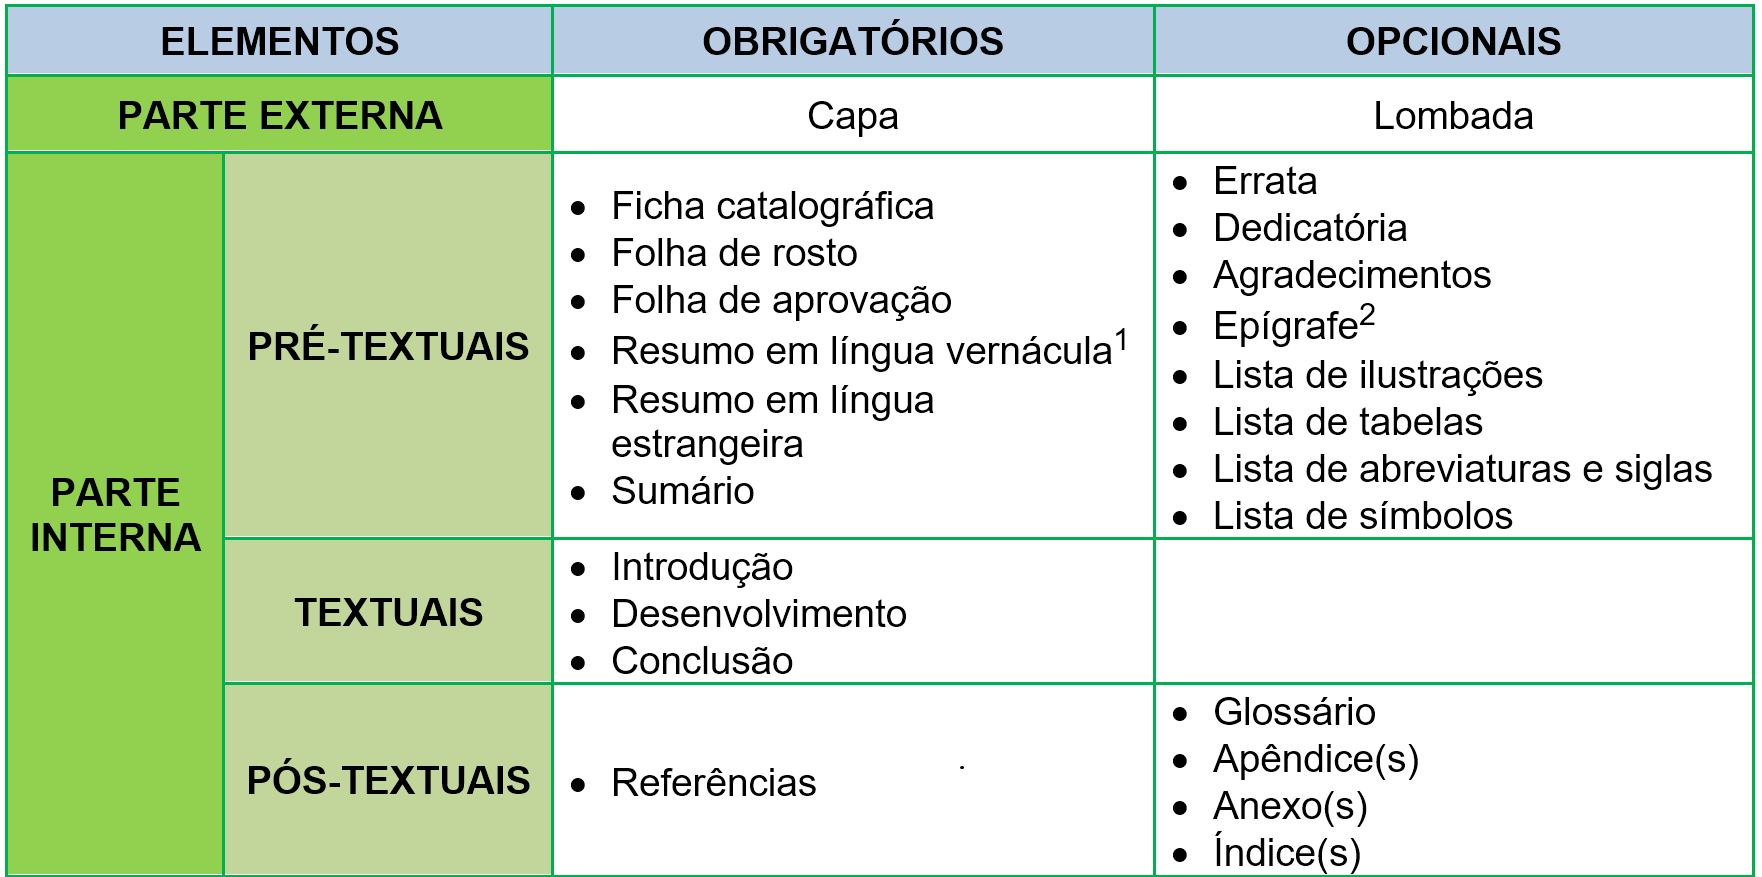
\includegraphics [width=1\textwidth] 
    {images/normaliza_ifb.png}
     \label{fig:Normaliza}
    \captionsetup{labelformat=empty}
    \caption*{Fonte: Normaliza IFB}
\end{figure}

Lembrando que cada indivíduo possui um lógica própria de organização de ideias, e cada orientador também possui uma visão sobre a produção de artefatos e execução de projetos, busco contribuir com o processo citando alguns trabalhos por mim orientados e compartilhando a seguir minhas observações acerca do detalhamento de conceitos e elaboração de textos que compõem um trabalho de conclusão de curso. 

\section{Elementos da Introdução}

Na introdução o trabalho deve trazer uma contextualização, uma explicação sobre qual é o tema que o trabalho irá tratar para alcançar o desenvolvimento (objetivos gerais e específicos) de uma solução ou produto. Nessa etapa é importante que o texto comece de forma ampla, com uma visão mais geral e depois vá se tornando mais especifico até chegar o ponto onde o assunto em questão será desenvolvido no projeto. A seguir são apresentados trechos de TCC´s com exeplos de citação de contexto amplo e mais específicos.

\begin{quote}
    "O mercado digital tem se popularizado cada vez mais nos últimos anos[...] segundo a empresa, o \textit{Wordpress}  constitui 43 por cento da \textit{WEB}. [...] A dinâmica da plataforma é utilizar os \textit{plugins} que existem nela para personalizar seu site de forma que atenda a sua demanda. \cite{marçal}
\end{quote}

\begin{quote}
    "A utilização de ferramentas para a leitura e processamento de grandes quantidades de dados[...] referente à epidemiologia de diferentes casos, é a próxima etapa desse processo de avanço tecnológico nos estudos epidemiológicos[...].A análise e tratamento das bases de dados que se formam dessas informações, nas quais são estudados os diferentes fatores que atuam na difusão e prevenção de doenças, é algo defendido pelos profissionais da área de epidemiologia" \cite{paulosilva}
    \end{quote}

As etapas de identificação de um tema busca contextualizar e justificar situações que devam ser tratada como problema ou oportunidade.  É possível  trazer neste capítulo um problema já conhecido, uma oportunidade ou uma questão bem definida, como por exemplo, um aplicativo que pode ser desenvolvido para resolver uma questão específica de uma empresa ou departamento de uma instituição.

A partir destas situações é possível definir  objetivos gerais e específicos como por exemplo: "desenvolver aplicação WEB que permitindo ao usuário direcionar seus investimentos em marketing e tráfego pago" ou "desenvolver ferramentas que permitam a mineração de dados de fontes diferentes por meio de web scraping, crawlers, e APIs públicas". 


\subsection{Objetivos geral e específico}

É a resposta ao problema especificado acima, ou seja, aquilo que se pretende fazer e que, depois de atingido, estará concluído o trabalho.

Para escrever bons objetivos \cite{doran} sugere que utilizemos o método \textit{\ac{smart}} buscando trazer informações específicas (S), que possam ser medidas (M), atribuídas (A) de maneira individual, realistas (R) e dentro de um limite de tempo (T).

O objetivo geral é mais amplo e sintetiza a meta do seu trabalho enquanto objetivos específicos trazem etapas e atividades que serão detalhadas e desenvolvidas no seu trabalho. É comum que alguns objetivos sejam ajustados na qualificação do projeto e também muito frequente que alguns objetivos não sejam alcançados, isto não é necessariamente demérito do aluno e deve ter suas causa explicadas nos resultados.       

Com objetivos estabelecidos serão explicados conceitos relacionados ao tema, metodologias aplicadas e as tecnologias utilizadas para o alcances destes objetivos bem como o relato do desenvolvimento de artefatos e resultados obtidos. 



 \subsection{Reflexão}
 O que se busca entender neste capítulo é se o escopo do projeto está bem definido, se os objetivos  que o estudante se propõe a fazer estão suficientemente bem definidos, são relevantes e se o projeto não está muito amplo, ou seja, se é possível realizar o que está se propondo em um semestre, que é o tempo disponível para execução do trabalho dentro da conclusão do curso.

Para encontrar um tema tenha em mente que você se compromete com o aprendizado e domínio do assunto e que o tema será lhe acompanhará durante a construção todo o trabalho, observe sua motivação em explicar e desenvolver algo nesse tema. Pense se é algo que você gostaria de ter lido ou feito e pense o quanto este trabalho realmente lhe será interessante. Lembre também que será preciso conversar com pessoas para levantar requisitos e/ou testar seus protótipos. 